\section{Notationen}
	\subsection{Charakteristische Funktion}
	Die charakteristische Funktion einer Menge $A \subset \R^n$ ist gegeben durch:
	\begin{equation}
		\textsl{x}_A(x) = 
		\begin{cases}
			1 \qquad, x \in A\\
			0 \qquad, x \in \R^n_{\backslash A}
		\end{cases}
	\end{equation}
	
	Dabei gilt
	\begin{equation}
		\textsl{x}_A \cdot \textsl{x}_B = \textsl{x}_{A \cap B}
	\end{equation}
	
	\subsection{Kartesisches Produkt}
	\begin{equation}
		A \times B = \lbrace (a,b)| a \in A, b \in B \rbrace
	\end{equation}
	
	\subsection{Infimum/Supremum}
	Das Infimum einer Menge ist die größte untere Schranke, das Supremum die kleinste obere Schranke. Schreibweise:
	\begin{align}
		\inf_{x\in A} A \\
		\sup_{x \in B} B
	\end{align}
	\newpage
	\subsection{Randpunkt und Rand}
	Ein Randpunkt $a$ von $A \subset \R^n$ ist ein Punkt $a \in \R^n$ mit
	\begin{align}
		B_\varepsilon (a) \cap A \neq 0\\
		B_\varepsilon (a) \cap A^c \neq 0
	\end{align}
	für alle $\varepsilon > 0$. Der Rand $\partial A$ von $A$ ist die Menge aller Randpunkte.
	  \begin{figure}[H] 
		  \centering
		  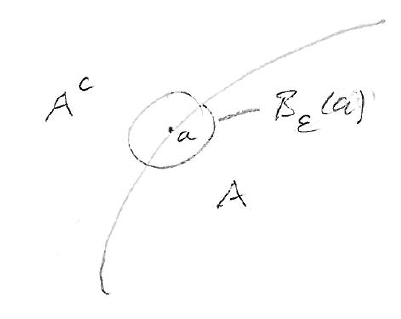
\includegraphics[width=0.5\textwidth]{./img/mass_randpunkte.png}
		  \caption{Randpunkte \protect\cite{HM3}}
		  \label{fig:randpunkte}
	  \end{figure}

\subsection{Nützliche Hilfssätze}
	\subsubsection{Reduktionsformel Sinus}
	\begin{equation}
		\int_a^b \sin^n(x) \dx =
\frac{n-1}{n}\int_a^b \sin^{n-2}(x)\dx \quad, a,b \in \frac{\pi}{2} \cdot \Z
	\end{equation}		  
	
		
	